\documentclass[a4paper, 11pt]{article}           %{{{1
% basic packages                                  {{{2
\usepackage[T1]{fontenc}
\usepackage[scaled=0.975]{helvet}
\usepackage[utf8]{inputenc}
\usepackage{amsmath}
\usepackage{lastpage}
\usepackage{graphicx}
\usepackage{amsfonts}
\usepackage{variations}
\usepackage{pgf,tikz}           % dessin
\usepackage{mathrsfs}
\usetikzlibrary{arrows}
\usepackage{pgfkeys}        % fenetrage des plot TikZ
\usepackage{yhmath}         % arc au dessus des lettres
\usepackage{calc}           % calcul de longueur
\usepackage{variations}     % tableau de variations
\usepackage{multicol}
\usepackage{enumitem}
%\usepackage{listings}       % syntax highlightingn of most common languages
%\usepackage{color}
%}}}

% mise en page                                    {{{2
\addtolength{\voffset}{-1.8cm}
\addtolength{\textheight}{4cm}
\addtolength{\hoffset}{-2.5cm}
\addtolength{\textwidth}{4cm}
\addtolength{\headsep}{-0.5cm}
\usepackage{fancyhdr}
\setlength{\headheight}{14.00pt}
\pagestyle{fancy} % Numérotation des pages
\renewcommand\headrulewidth{1pt}
\fancyhead[L]{2nd SN}
\fancyhead[C]{bloc alimentation autonome}
\fancyhead[R]{\textbf{Habitat intelligent}}
\renewcommand\footrulewidth{1pt}
\fancyfoot[L]{v 1.0 - non testé}
\fancyfoot[C]{octobre 2017}
\fancyfoot[R]{\thepage/\pageref{LastPage}}
%\lhead{3E}%haut de page gauche
%}}}

% Compteurs:                                     {{{2
\addtocounter{page}{0}
\newcounter{Q}
\newcounter{exoNB}
%}}}

% Longueur:                                      {{{2
\newlength{\longueurA}
\newlength{\longueurB}
\setlength{\parindent}{0pt}
\setlength{\parskip}{2pt}
\renewcommand{\baselinestretch}{1}
%}}}

% Divers                                          {{{2
% listings                                        {{{3
%\definecolor{mygreen}{rgb}{0,0.6,0}
%\definecolor{mygray}{rgb}{0.5,0.5,0.5}
%\definecolor{mymauve}{rgb}{0.58,0,0.82}
%\definecolor{deepblue}{rgb}{0,0,0.5}
%\definecolor{deepred}{rgb}{0.6,0,0}
%\definecolor{deepgreen}{rgb}{0,0.5,0}
%\lstset{%
%        backgroundcolor=\color{white},   % choose the background color; you must add \usepackage{color} or \usepackage{xcolor}; should come as last argument
%        basicstyle=\footnotesize,        % the size of the fonts that are used for the code
%        breakatwhitespace=false,         % sets if automatic breaks should only happen at whitespace
%        breaklines=true,                 % sets automatic line breaking
%        captionpos=b,                    % sets the caption-position to bottom
%        commentstyle=\color{mygreen},    % comment style
%        deletekeywords={...},            % if you want to delete keywords from the given language
%        escapeinside={\%*}{*)},          % if you want to add LaTeX within your code
%        extendedchars=true,              % lets you use non-ASCII characters; for 8-bits encodings only, does not work with UTF-8
%        frame=single,                    % adds a frame around the code
%        keepspaces=true,                 % keeps spaces in text, useful for keeping indentation of code (possibly needs columns=flexible)
%        keywordstyle=\color{blue},       % keyword style
%        morekeywords={*,...},            % if you want to add more keywords to the set
%        numbers=left,                    % where to put the line-numbers; possible values are (none, left, right)
%        numbersep=5pt,                   % how far the line-numbers are from the code
%        numberstyle=\tiny\color{mygray}, % the style that is used for the line-numbers
%        rulecolor=\color{black},         % if not set, the frame-color may be changed on line-breaks within not-black text (e.g. comments (green here))
%        showspaces=false,                % show spaces everywhere adding particular underscores; it overrides 'showstringspaces'
%        showstringspaces=false,          % underline spaces within strings only
%        showtabs=false,                  % show tabs within strings adding particular underscores
%        stepnumber=2,                    % the step between two line-numbers. If it's 1, each line will be numbered
%        stringstyle=\color{mymauve},     % string literal style
%        tabsize=4,                       % sets default tabsize to 2 spaces
%        title=\lstname                   % show the filename of files included with \lstinputlisting; also try caption instead of title
%}
%\lstset{%
%        language=Python,                 % the language of the code
%        otherkeywords={self},            % Add keywords here
%        deletekeywords={type},           % if you want to delete keywords from the given language
%        emph={},                         % Custom highlighting
%        emphstyle=\ttb\color{deepred}    % Custom highlighting style
%}
%}}}

% PRL style line                                 {{{3
\newlength{\diamondrulelength}
\setlength{\diamondrulelength}{0.6\textwidth}
\newlength{\diamondrulethickness}
\setlength{\diamondrulethickness}{2pt}
\newcommand{\diamondrule}{\begin{center}\tikz{\fill[black] (0.5\diamondrulelength,0) -- (0,0.5\diamondrulethickness) -- (-0.5\diamondrulelength,0) -- (0,-0.5\diamondrulethickness) -- cycle;}\end{center}}
%}}}

% fixed with tabular                             {{{3
\usepackage{array}
\newcolumntype{L}[1]{>{\raggedright\let\newline\\\arraybackslash\hspace{0pt}}m{#1}}
\newcolumntype{C}[1]{>{\centering\let\newline\\\arraybackslash\hspace{0pt}}m{#1}}
\newcolumntype{R}[1]{>{\raggedleft\let\newline\\\arraybackslash\hspace{0pt}}m{#1}}
%}}}

%}}}
%}}}

\begin{document}
\sffamily

% https://www.allaboutcircuits.com/projects/create-an-arduino-controlled-battery-charger/
% https://circuitdigest.com/electronic-circuits/emergency-light-circuit

\begin{center}
\textsc{Bloc Autonome d'Eclairage de Sécurité : BAES}\\
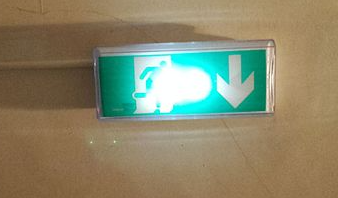
\includegraphics[width=0.6\textwidth]{BAES}
\end{center}
Les blocs autonomes d'éclairage de sécurité (BAES), parfois appelés « Blocs de secours », sont des sources lumineuses d'évacuation destinées à éclairer et montrer l'emplacement des sorties dans différents types d'établissement lors d'évacuation d'urgence ou de défaillance de l'éclairage principal d'un bâtiment. Ils permettent de respecter la législation et les règles d'usages pour les locaux accueillant le public.

Ces blocs sont constitués d'un luminaire muni d'ampoules et d'une batterie, le tout permettant d'assurer un fonctionnement pendant une durée déterminée par les codes ou règlements locaux/nationaux. Cette durée est généralement d'une heure en Europe et de trente minutes en Amérique du Nord.

\textsc{Chargeur de batterie}\\

\begin{center}
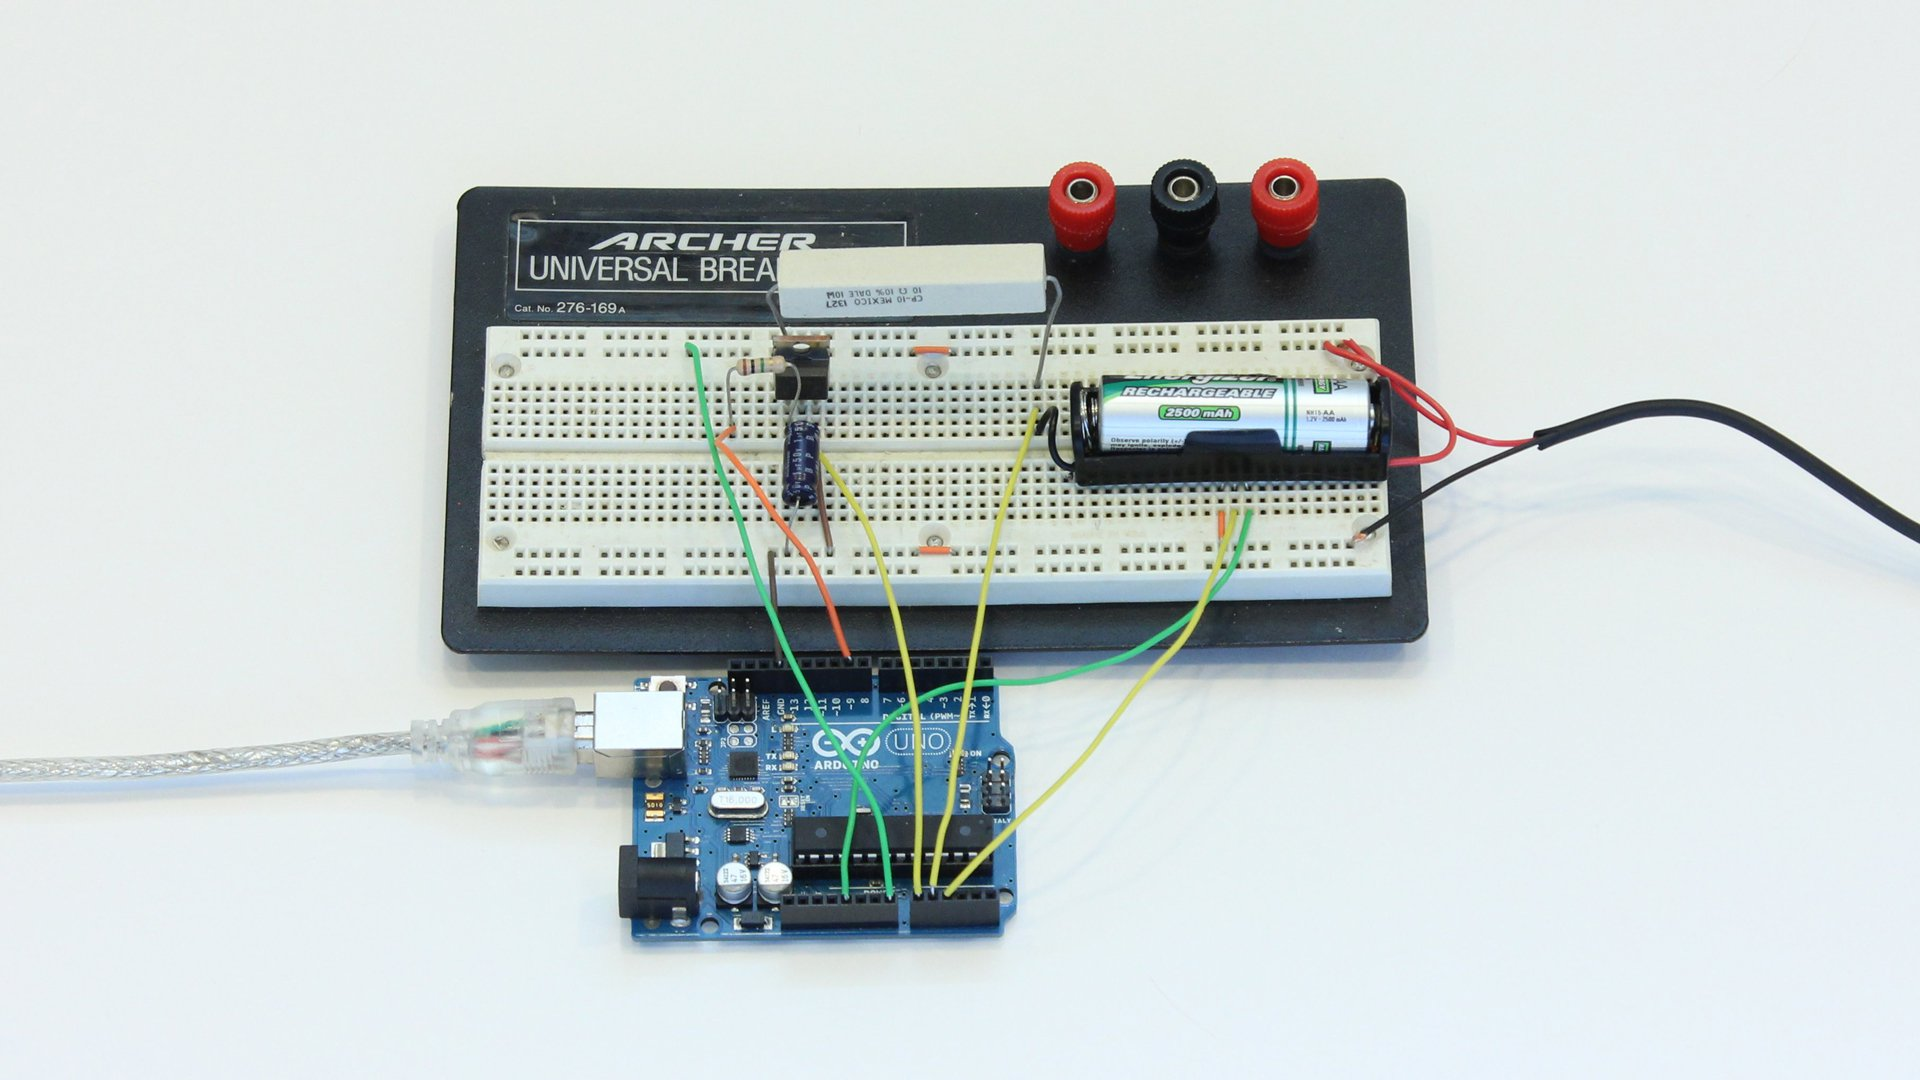
\includegraphics[width=0.6\textwidth]{chargeur_realisation}
\end{center}

{\bf Composants}
\begin{itemize}
\item Arduino Microcontroller
\item 3 AA Battery Holder
\item NiMH AA Battery
\item 10 ohm Power Resistor (rated for at least 5 watts)
\item 1 Mohm resistor
\item 1 uF Capacitor
\item IRF510 MOSFET
\item TMP36 Temperature Sensor
\item 5V Regulated Power Supply
\item Prototyping Breadboard
\item Jumper Wires
\end{itemize}

\begin{center}
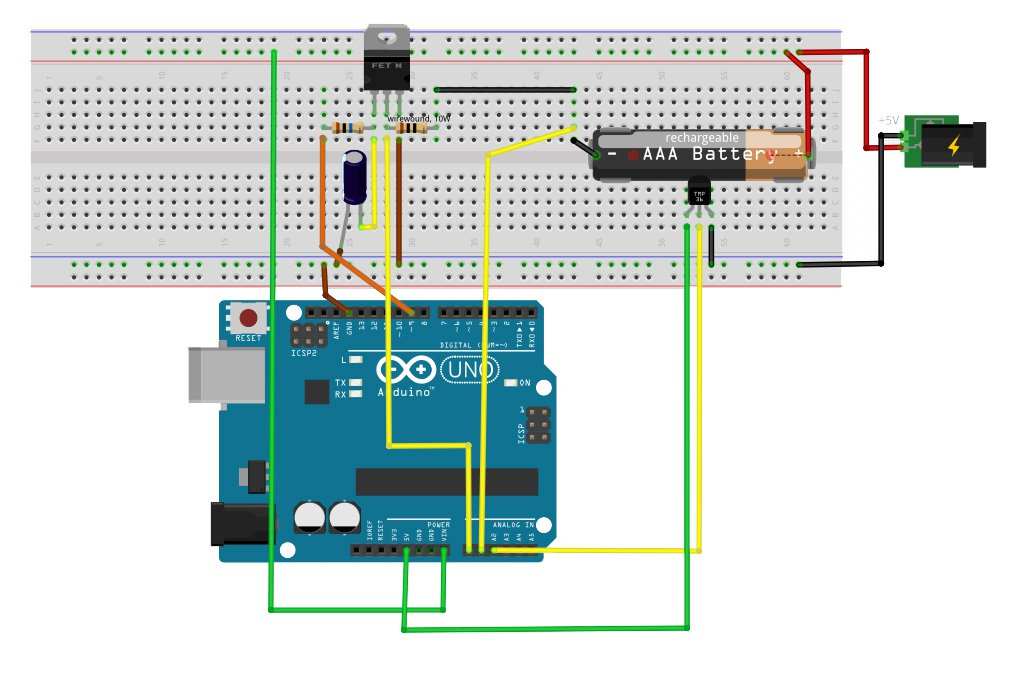
\includegraphics[width=0.45\textwidth]{arduino_battery_charger_diagram}
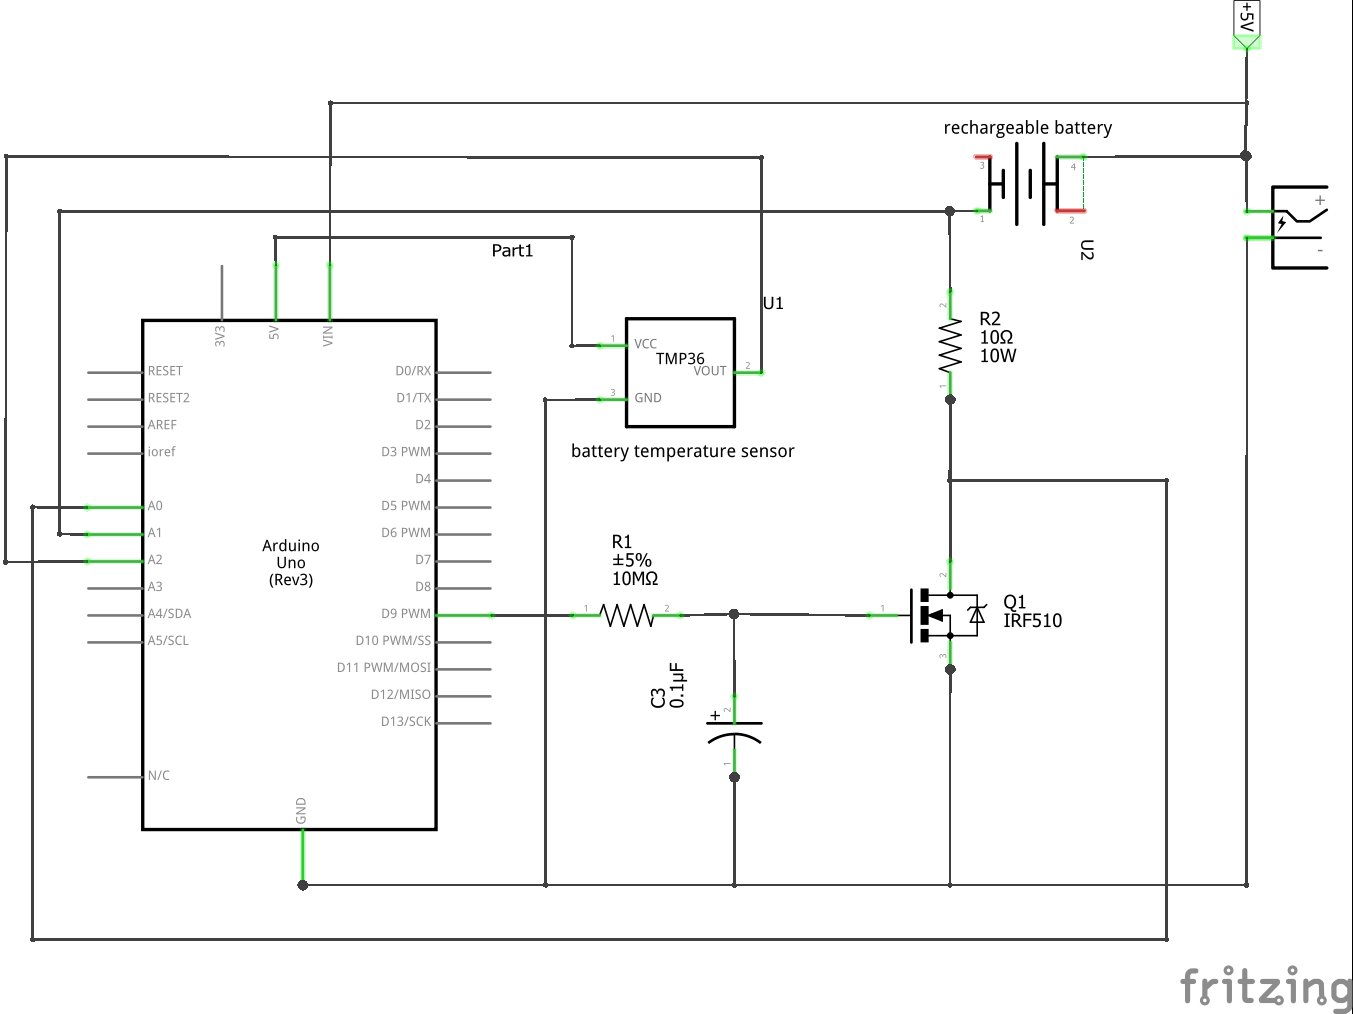
\includegraphics[width=0.45\textwidth]{arduino_battery_charger_schem}
\end{center}

\stepcounter{Q}$\boxed{\arabic{Q}}$ Réaliser le montage ci-dessus. \\
Constation professeur :

\stepcounter{Q}$\boxed{\arabic{Q}}$ Implémenter le code ci-dessous. \\
Constation professeur :

\stepcounter{Q}$\boxed{\arabic{Q}}$ Tester le code ci-dessous. \\
Constation professeur :

\scriptsize %{{{1
\begin{verbatim}
int batteryCapacity = 2500;     //capacity rating of battery in mAh
float resistance = 10.0;     //measured resistance of the power resistor
int cutoffVoltage = 1600;     //maximum battery voltage (in mV) that should not be exceeded
float cutoffTemperatureC = 35;     //maximum battery temperature that should not be exceeded (in degrees C)
//float cutoffTemperatureF = 95;     //maximum battery temperature that should not be exceeded (in degrees F)
long cutoffTime = 46800000;     //maximum charge time of 13 hours that should not be exceeded

int outputPin = 9;     // Output signal wire connected to digital pin 9
int outputValue = 150;     //value of PWM output signal

int analogPinOne = 0;     //first voltage probe connected to analog pin 1
float valueProbeOne = 0;     //variable to store the value of analogPinOne
float voltageProbeOne = 0;     //calculated voltage at analogPinOne

int analogPinTwo = 1;     //second voltage probe connected to analog pin 2
float valueProbeTwo = 0;     //variable to store the value of analogPinTwo
float voltageProbeTwo = 0;     //calculated voltage at analogPinTwo

int analogPinThree = 2;     //third voltage probe connected to analog pin 2
float valueProbeThree = 0;     //variable to store the value of analogPinThree
float tmp36Voltage = 0;     //calculated voltage at analogPinThree
float temperatureC = 0;     //calculated temperature of probe in degrees C
//float temperatureF = 0;     //calculated temperature of probe in degrees F

float voltageDifference = 0;     //difference in voltage between analogPinOne and analogPinTwo
float batteryVoltage = 0;     //calculated voltage of battery
float current = 0;     //calculated current through the load (in mA)
float targetCurrent = batteryCapacity / 10;     //target output current (in mA) set at C/10 or 1/10 of the battery capacity per hour
float currentError = 0;     //difference between target current and actual current (in mA)



void setup()
{
  Serial.begin(9600);     //  setup serial
  pinMode(outputPin, OUTPUT);     // sets the pin as output
}



void loop()
{

  analogWrite(outputPin, outputValue);  //Write output value to output pin

  Serial.print("Output: ");     //display output values for monitoring with a computer
  Serial.println(outputValue);

  valueProbeOne = analogRead(analogPinOne);    // read the input value at probe one
  voltageProbeOne = (valueProbeOne*5000)/1023;     //calculate voltage at probe one in milliVolts
  Serial.print("Voltage Probe One (mV): ");     //display voltage at probe one
  Serial.println(voltageProbeOne);

  valueProbeTwo = analogRead(analogPinTwo);    // read the input value at probe two
  voltageProbeTwo = (valueProbeTwo*5000)/1023;     //calculate voltage at probe two in milliVolts
  Serial.print("Voltage Probe Two (mV): ");     //display voltage at probe two
  Serial.println(voltageProbeTwo);

  batteryVoltage = 5000 - voltageProbeTwo;     //calculate battery voltage
  Serial.print("Battery Voltage (mV): ");     //display battery voltage
  Serial.println(batteryVoltage);

  current = (voltageProbeTwo - voltageProbeOne) / resistance;     //calculate charge current
  Serial.print("Target Current (mA): ");     //display target current
  Serial.println(targetCurrent);
  Serial.print("Battery Current (mA): ");     //display actual current
  Serial.println(current);

  currentError = targetCurrent - current;     //difference between target current and measured current
  Serial.print("Current Error  (mA): ");     //display current error
  Serial.println(currentError);

  valueProbeThree = analogRead(analogPinThree);    // read the input value at probe three
  tmp36Voltage = valueProbeThree * 5.0;     // converting that reading to voltage
  tmp36Voltage /= 1024.0;

  temperatureC = (tmp36Voltage - 0.5) * 100 ;     //converting from 10 mv per degree wit 500 mV offset to degrees ((voltage - 500mV) times 100)
  Serial.print("Temperature (degrees C) ");     //display the temperature in degrees C
  Serial.println(temperatureC);

 /*
  temperatureF = (temperatureC * 9.0 / 5.0) + 32.0;     //convert to Fahrenheit
  Serial.print("Temperature (degrees F) ");
  Serial.println(temperatureF);
 */

  Serial.println();     //extra spaces to make debugging data easier to read
  Serial.println();



  if(abs(currentError) > 10)     //if output error is large enough, adjust output
   {
    outputValue = outputValue + currentError / 10;

    if(outputValue < 1)    //output can never go below 0
     {
      outputValue = 0;
     }

    if(outputValue > 254)     //output can never go above 255
     {
      outputValue = 255;
     }

    analogWrite(outputPin, outputValue);     //write the new output value
   }


  if(temperatureC > cutoffTemperatureC)     //stop charging if the battery temperature exceeds the safety threshold
   {
    outputValue = 0;
    Serial.print("Max Temperature Exceeded");
   }

  /*
  if(temperatureF > cutoffTemperatureF)     //stop charging if the battery temperature exceeds the safety threshold
   {
    outputValue = 0;
   }
   */

   if(batteryVoltage > cutoffVoltage)     //stop charging if the battery voltage exceeds the safety threshold
   {
    outputValue = 0;
    Serial.print("Max Voltage Exceeded");
   }

   if(millis() > cutoffTime)     //stop charging if the charge time threshold
   {
    outputValue = 0;
    Serial.print("Max Charge Time Exceeded");
   }

   delay(10000);     //delay 10 seconds before next iteration
}
\end{verbatim} %}}}
\normalsize


\textsc{Alimentation d'urgence}\\
\begin{center}
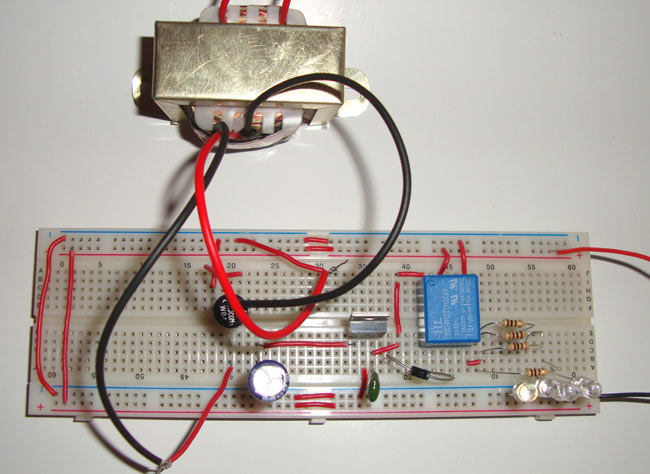
\includegraphics[width=0.6\textwidth]{Emergency-Light}
\end{center}
{\bf Composants}
\begin{itemize}
\item Transformer- 9-0-9 500mA
\item Bridge rectifier
\item Diode- 1N4007
\item IC 7808 voltage regulator
\item Capacitor 1000uF, 0.01uF
\item Relay- 6v
\item Resistors- 100 ohm
\item LEDs- Ultra bright white LED
\item Rechargeable 6v, 4.5Ah Battery
\end{itemize}

\begin{center}
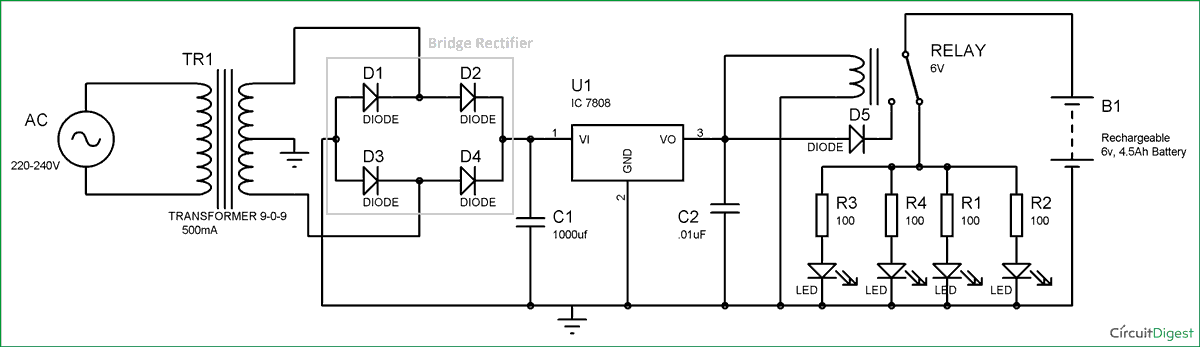
\includegraphics[width=\textwidth]{emergency-light-circuit}
\end{center}

\stepcounter{Q}$\boxed{\arabic{Q}}$ Connecter juste le transformateur du montage ci-dessus. Mesurer la tension.\\
Constation professeur :

\stepcounter{Q}$\boxed{\arabic{Q}}$ Connecter le transformateur et le pont de diodes du montage ci-dessus. Mesurer la tension. \\
Constation professeur :

\stepcounter{Q}$\boxed{\arabic{Q}}$ Connecter le transformateur, le pont de diodes et le regulateur du montage ci-dessus. Mesurer la tension.\\
Constation professeur :

\stepcounter{Q}$\boxed{\arabic{Q}}$ Connecter le transformateur, le pont de diodes, le regulateur et le relai avec sa diode de protection du montage ci-dessus. Mesurer la tension.\\
Constation professeur :

\vspace{1cm}
\textsc{BAES}\\

\stepcounter{Q}$\boxed{\arabic{Q}}$ Représenter un diagramme de fonctionnement combinant les deux circuits précédents et réalisant un BAES. \\
Constation professeur :


\stepcounter{Q}$\boxed{\arabic{Q}}$ Connecter les deux parties du circuit et réaliser le BAES. \\
Constation professeur :




\end{document}
%vim:fdm=marker

